\documentclass[10pt,xcolor=svgnames]{beamer} %Beamer
\usepackage{palatino} %font type
\usefonttheme{metropolis} %Type of slides
\usefonttheme[onlymath]{serif} %font type Mathematical expressions
\usetheme[progressbar=frametitle,titleformat frame=smallcaps,numbering=counter]{metropolis} %This adds a bar at the beginning of each section.
\useoutertheme[subsection=false]{miniframes} %Circles in the top of each frame, showing the slide of each section you are at

\usepackage{appendixnumberbeamer} %enumerate each slide without counting the appendix
\setbeamercolor{progress bar}{fg=Maroon!70!Coral} %These are the colours of the progress bar. Notice that the names used are the svgnames
\setbeamercolor{title separator}{fg=DarkSalmon} %This is the line colour in the title slide
\setbeamercolor{structure}{fg=black} %Colour of the text of structure, numbers, items, blah. Not the big text.
\setbeamercolor{normal text}{fg=black!87} %Colour of normal text
\setbeamercolor{alerted text}{fg=DarkRed!60!Gainsboro} %Color of the alert box
\setbeamercolor{example text}{fg=Maroon!70!Coral} %Colour of the Example block text


\setbeamercolor{palette primary}{bg=NavyBlue!50!DarkOliveGreen, fg=white} %These are the colours of the background. Being this the main combination and so one. 
\setbeamercolor{palette secondary}{bg=NavyBlue!50!DarkOliveGreen, fg=white}
\setbeamercolor{palette tertiary}{bg=NavyBlue!40!Black, fg= white}
\setbeamercolor{section in toc}{fg=NavyBlue!40!Black} %Color of the text in the table of contents (toc)

\usepackage{multicol}

\newcounter{countitems}
\newcounter{nextitemizecount}
\newcommand{\setupcountitems}{%
  \stepcounter{nextitemizecount}%
  \setcounter{countitems}{0}%
  \preto\item{\stepcounter{countitems}}%
}
\makeatletter
\newcommand{\computecountitems}{%
  \edef\@currentlabel{\number\c@countitems}%
  \label{countitems@\number\numexpr\value{nextitemizecount}-1\relax}%
}
\newcommand{\nextitemizecount}{%
  \getrefnumber{countitems@\number\c@nextitemizecount}%
}
\newcommand{\previtemizecount}{%
  \getrefnumber{countitems@\number\numexpr\value{nextitemizecount}-1\relax}%
}
\makeatother    
\newenvironment{AutoMultiColItemize}{%
\ifnumcomp{\nextitemizecount}{>}{3}{\begin{multicols}{2}}{}%
\setupcountitems\begin{itemize}}%
{\end{itemize}%
\unskip\computecountitems\ifnumcomp{\previtemizecount}{>}{3}{\end{multicols}}{}}

%These next packages are the useful for Physics in general, you can add the extras here. 
\usepackage{amsmath,amssymb}
\usepackage{slashed}
\usepackage{cite}
\usepackage{relsize}
\usepackage{caption}
\usepackage{subcaption}
\usepackage{multicol}
\usepackage{booktabs}
\usepackage[scale=2]{ccicons}
\usepackage{pgfplots}
\usepgfplotslibrary{dateplot}
\usepackage{geometry}
\usepackage{xspace}
\newcommand{\themename}{\textbf{\textsc{bluetemp}\xspace}}%metropolis}}\xspace}

\title{Artigo \\ Modelagem de Fenômenos Biológicos}
\author[Name]{Raphael Levy e Erick Brito \\ Orientador: Flávio Coelho} %With inst, you can change the institution they belong
\date{}
\subtitle{Quimiostato}
\institute[uni]{EMAP - FGV}

%%% logo aqui
%\titlegraphic{\vspace{-0.5cm}\hfill
\includegraphics[scale=0.23]{logo.png}} %You can modify the location of the logo by changing the command \vspace{}. 

\begin{document}
{
\setbeamercolor{background canvas}{bg=NavyBlue!50!DarkOliveGreen, fg=white}
\setbeamercolor{normal text}{fg=white}
\maketitle
}%This is the colour of the first slide. bg= background and fg=foreground

\metroset{titleformat frame=smallcaps} %This changes the titles for small caps

\begin{frame}{Sumário}
  \setbeamertemplate{section in toc}[sections numbered] %This is numbering the sections
  \tableofcontents[hideallsubsections] %You can comment this line if you want to show the subsections in the table of contents
\end{frame}

%\begin{frame}{Objectives}
%\underline{\textsc{Some text:}}
%\begin{small}
%This is some small Text. 
%\end{small}

%\metroset{block=fill}
%\begin{exampleblock}{\textsc{Example block}}
%\begin{itemize}
%    \item You know how to do itemize
%    \item Also here
%\end{itemize}
%\end{exampleblock}
%\end{frame}


\section{Introdução}

\begin{frame}[fragile]{Quimiostato} %You can change fragile by standout
\begin{figure}[H]
        \centering
        \hbox{\hspace{5.0em} 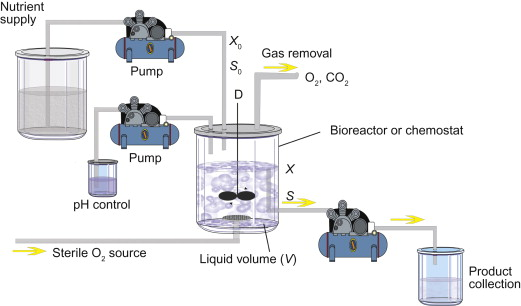
\includegraphics[scale=0.7] {Funcionamento_Quimiostato.jpg}} 
        \caption*{Funcionamento de um quimiostato}
\end{figure}
\end{frame}


\begin{frame}[standout]{Equação de Monod}
\begin{equation*}
    \mu = \mu_{max} \frac{[S]}{K_s + [S]}
\end{equation*}
\end{frame}

%\section[Outsider section]{Exotic section}

\begin{frame}{Hello}
    You can actually include a new section outside and edit apart.
\end{frame}

\section{Metodologia}
\begin{frame}{Modelo de Monod} %You can also not write fragile or standout and you can see how it looks
No modelo de Monod utilizamos as seguintes equações:
\begin{align}
  (dX/dt) &= \mu X-DX \\
  (dS/dt) &= DS_f-DS-(\mu X/Y)\\
  \mu &= \mu_{max}S/(K_s+S)\\
  D &\leq \mu_{max}S_f/(K_s + S_f)
\end{align}
Com
\begin{itemize}
\item $X$ = Concentração de massa celular (Massa/Volume)
\item $S$ = Limite de concentração de saída do substrato (Massa/Volume)
\item $S_f$ = Limite de concentração de entrada do substrato (Massa/Volume)
\item $D$ = Taxa de diluição (1/Tempo)
\end{itemize}
\end{frame}

\begin{frame}{Modelo de Monod}
\begin{itemize}
    \item $\mu$ = Taxa de crescimento específica (1/Tempo)
    \item $\mu_{max}$ = Máxima taxa de crescimento específica (1/Tempo)
    \item $Y$ = Coeficiente de rendimento (Massa celular/Massa do substrato limitante)
    \item $K_s$ = Constante de saturação (Massa/Volume)
\end{itemize}

\end{frame}

\section{Resultados}
\begin{frame}{Equações de estado estacionário} %You can also not write fragile or standout and you can see how it looks
A partir de certos valores de $X$ e $S$, as retas passam a ser constantes. Esses valores podem ser calculados através das seguintes equações:
\begin{align}
  S &= Ks*D/(\mu_{max}-D) \\
  X &= Y*(Sf- Ks*D/(\mu_{max}-D))
\end{align}
\end{frame}

\begin{frame}{}
\begin{figure}[H]
        \centering
        \hbox{\hspace{0.0em} 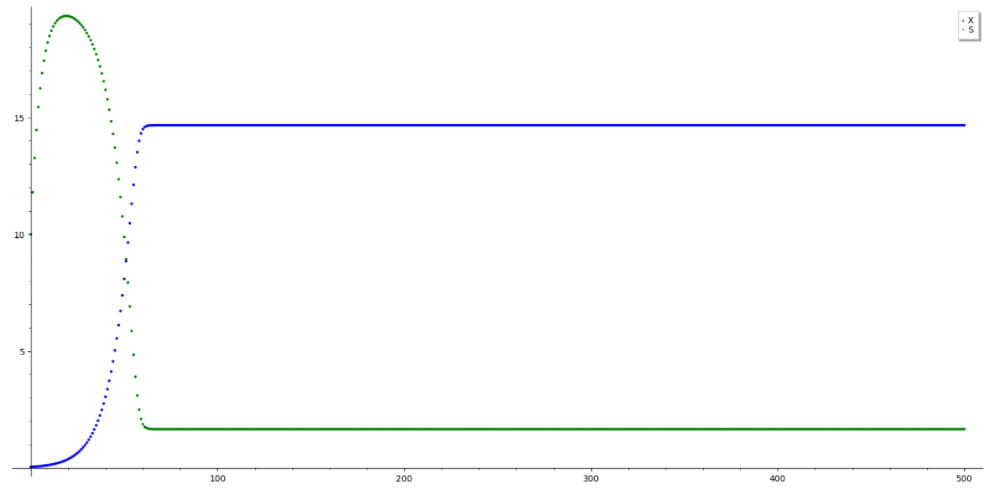
\includegraphics[scale=0.4]{Modelo_1.png}} 
        \caption*{Parâmetros originais}
\end{figure}
\vspace{-7mm}
\begin{itemize}
\begin{AutoMultiColItemize}
    \item $\mu_{max} = 1.6$ \\
    \item $K_s = 1.0$ \\
    \item $Y = 0.8$ \\
    \item $S_f = 20$ \\
    \item $D = 1.0$ \\
    \item $X_0 = 0.05$ \\
    \item $S_0 = 10.0$ \\
    \item $\mu = 1.0$
\end{AutoMultiColItemize}
\end{itemize}    
\end{frame}

\begin{frame}{}
\begin{figure}[H]
        \centering
        \hbox{\hspace{0.0em} 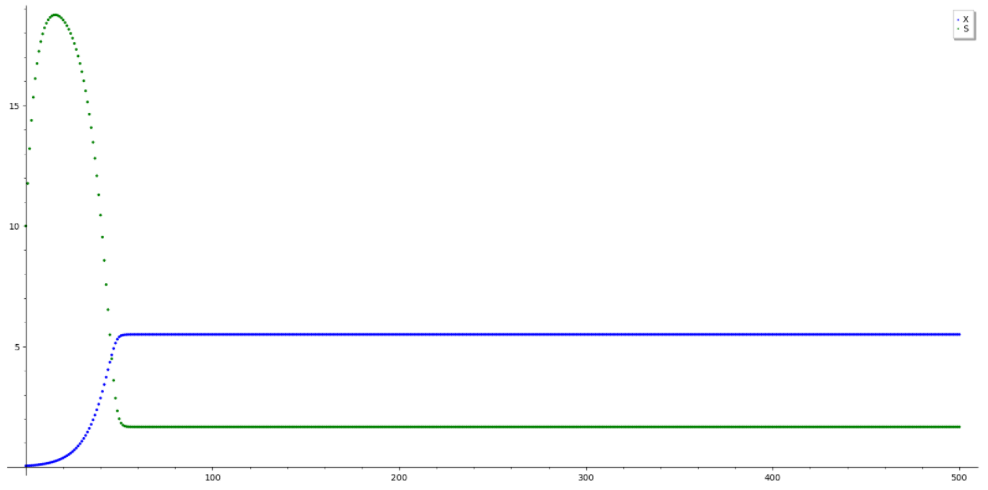
\includegraphics[scale=0.4]{Modelo_2.png}} 
        \caption*{Diminuindo o coeficiente de rendimento}
\end{figure}
\vspace{-7mm}
\begin{itemize}
\begin{AutoMultiColItemize}
    \item $\mu_{max} = 1.6$ \\
    \item $K_s = 1.0$ \\
    \item $Y = 0.3$ \\
    \item $S_f = 20$ \\
    \item $D = 1.0$ \\
    \item $X_0 = 0.05$ \\
    \item $S_0 = 10.0$ \\
    \item $\mu = 1.0$
\end{AutoMultiColItemize}
\end{itemize}
\end{frame}

\begin{frame}{}
\begin{figure}[H]
        \centering
        \hbox{\hspace{0.0em} 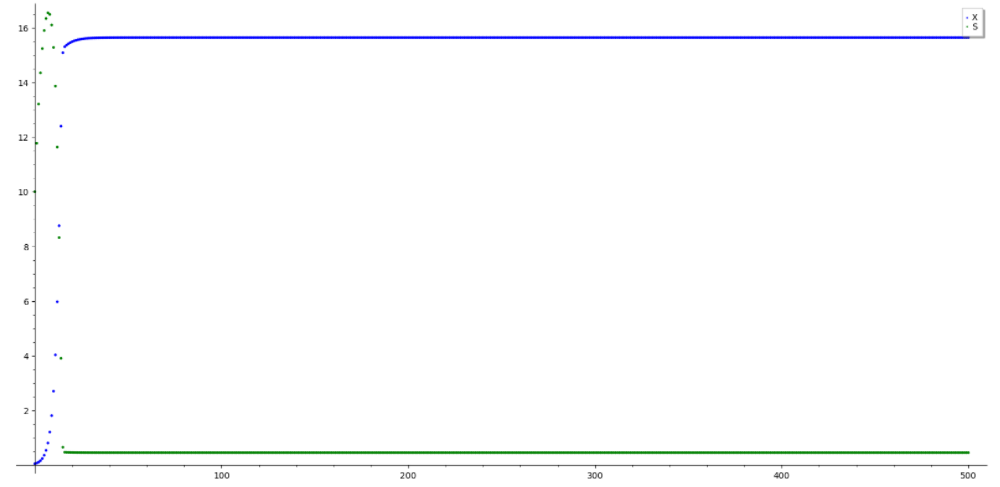
\includegraphics[scale=0.4]{Modelo_3.png}} 
        \caption*{Dobrando a taxa máxima de crescimento}
\end{figure}
\vspace{-7mm}
\begin{itemize}
\begin{AutoMultiColItemize}
    \item $\mu_{max} = 3.2$ \\
    \item $K_s = 1.0$ \\
    \item $Y = 0.8$ \\
    \item $S_f = 20$ \\
    \item $D = 1.0$ \\
    \item $X_0 = 0.05$ \\
    \item $S_0 = 10.0$ \\
    \item $\mu = 1.0$
\end{AutoMultiColItemize}
\end{itemize}
\end{frame}

\begin{frame}{}
\begin{figure}[H]
        \centering
        \hbox{\hspace{0.0em} 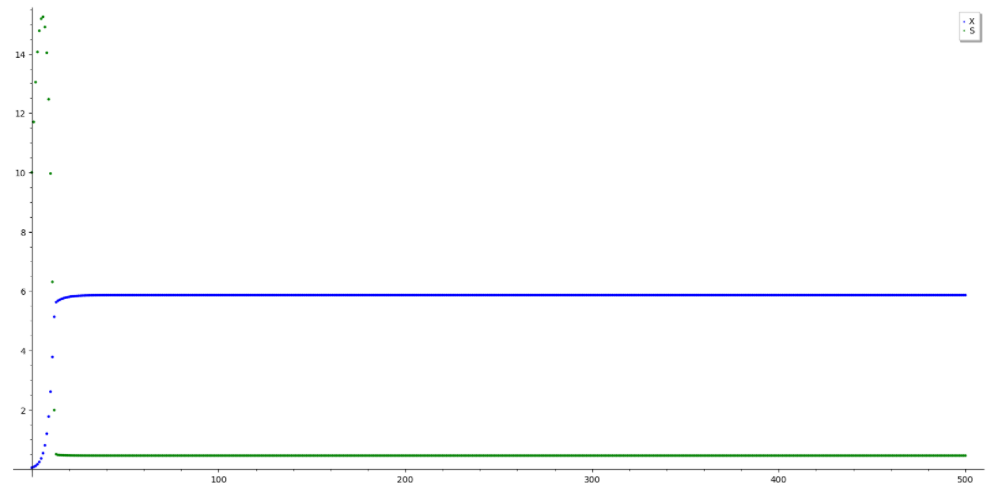
\includegraphics[scale=0.4]{Modelo_4.png}} 
        \caption*{Dobrando a taxa máxima de crescimento e diminuindo o coeficiente de rendimento}
\end{figure}
\vspace{-10mm}
\begin{itemize}
\begin{AutoMultiColItemize}
    \item $\mu_{max} = 3.2$ \\
    \item $K_s = 1.0$ \\
    \item $Y = 0.3$ \\
    \item $S_f = 20$ \\
    \item $D = 1.0$ \\
    \item $X_0 = 0.05$ \\
    \item $S_0 = 10.0$ \\
    \item $\mu = 1.0$
\end{AutoMultiColItemize}
\end{itemize}
\end{frame}

\begin{frame}{}
\begin{figure}[H]
        \centering
        \hbox{\hspace{0.0em} 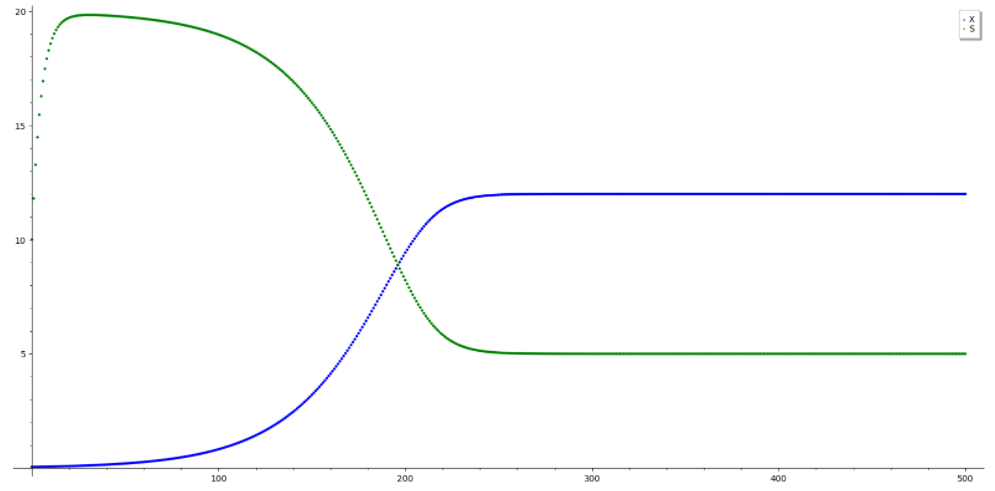
\includegraphics[scale=0.4]{Modelo_5_New.png}} 
        \caption*{Diminuindo a taxa máxima de crescimento}
\end{figure}
\vspace{-7mm}
\begin{itemize}
\begin{AutoMultiColItemize}
    \item $\mu_{max} = 1.2$ \\
    \item $K_s = 1.0$ \\
    \item $Y = 0.8$ \\
    \item $S_f = 20$ \\
    \item $D = 1.0$ \\
    \item $X_0 = 0.05$ \\
    \item $S_0 = 10.0$ \\
    \item $\mu = 1.0$
\end{AutoMultiColItemize}
\end{itemize}
\end{frame}

\begin{frame}{}
\begin{figure}[H]
        \centering
        \hbox{\hspace{0.0em} 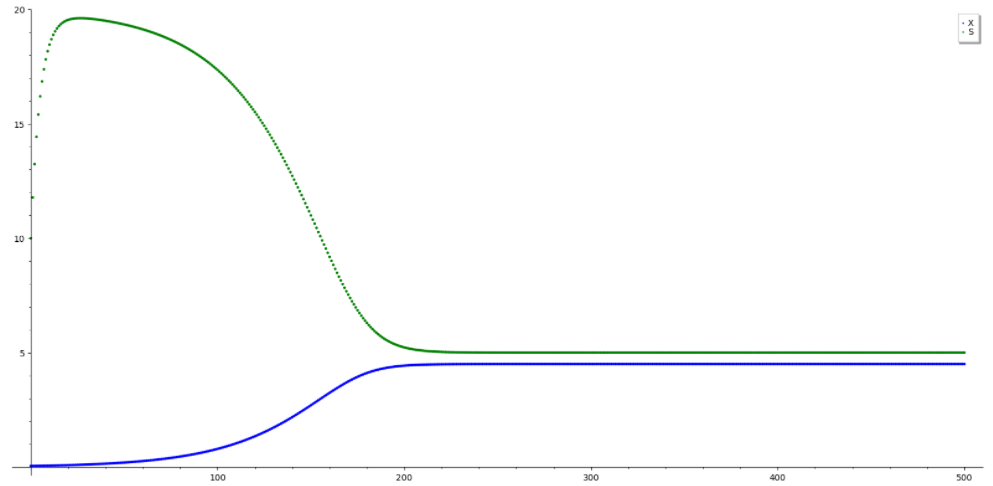
\includegraphics[scale=0.4]{Modelo_6_New.png}} 
        \caption*{Diminuindo a taxa máxima de crescimento e diminuindo o coeficiente de rendimento}
\end{figure}
\vspace{-10mm}
\begin{itemize}
\begin{AutoMultiColItemize}
    \item $\mu_{max} = 1.2$ \\
    \item $K_s = 1.0$ \\
    \item $Y = 0.3$ \\
    \item $S_f = 20$ \\
    \item $D = 1.0$ \\
    \item $X_0 = 0.05$ \\
    \item $S_0 = 10.0$ \\
    \item $\mu = 1.0$
\end{AutoMultiColItemize}
\end{itemize}
\end{frame}

\begin{frame}
\begin{figure}[H]
        \centering
        \hbox{\hspace{0.0em} 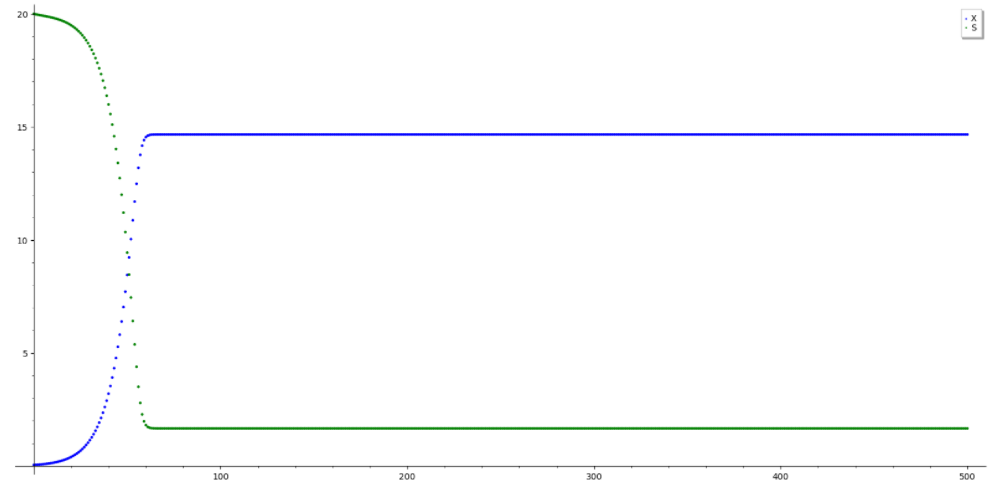
\includegraphics[scale=0.4]{Modelo_7.png}} 
        \caption*{Dobrando o limite de concentração de saída do substrato}
\end{figure}
\vspace{-7mm}
\begin{itemize}
\begin{AutoMultiColItemize}
    \item $\mu_{max} = 1.6$ \\
    \item $K_s = 1.0$ \\
    \item $Y = 0.8$ \\
    \item $S_f = 20$ \\
    \item $D = 1.0$ \\
    \item $X_0 = 0.05$ \\
    \item $S_0 = 20.0$ \\
    \item $\mu = 1.0$
\end{AutoMultiColItemize}
\end{itemize}
\end{frame}

\begin{frame}{}
\begin{figure}[H]
        \centering
        \hbox{\hspace{0.0em} 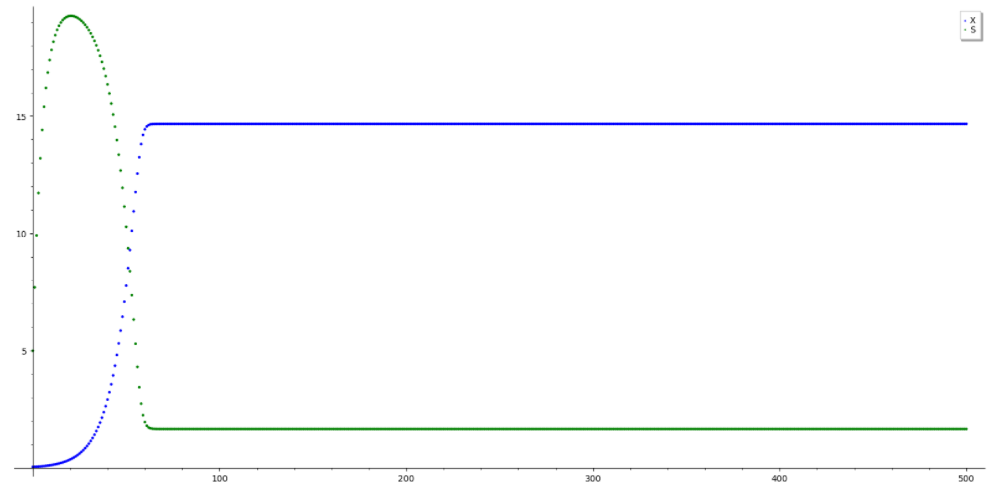
\includegraphics[scale=0.4]{Modelo_8.png}} 
        \caption*{Diminuindo o limite de concentração de saída do substrato pela metade}
\end{figure}
\vspace{-7mm}
\begin{itemize}
\begin{AutoMultiColItemize}
    \item $\mu_{max} = 1.6$ \\
    \item $K_s = 1.0$ \\
    \item $Y = 0.8$ \\
    \item $S_f = 20$ \\
    \item $D = 1.0$ \\
    \item $X_0 = 0.05$ \\
    \item $S_0 = 5.0$ \\
    \item $\mu = 1.0$
\end{AutoMultiColItemize}
\end{itemize}
\end{frame}

\begin{frame}
\begin{figure}[H]
        \centering
        \hbox{\hspace{0.0em} 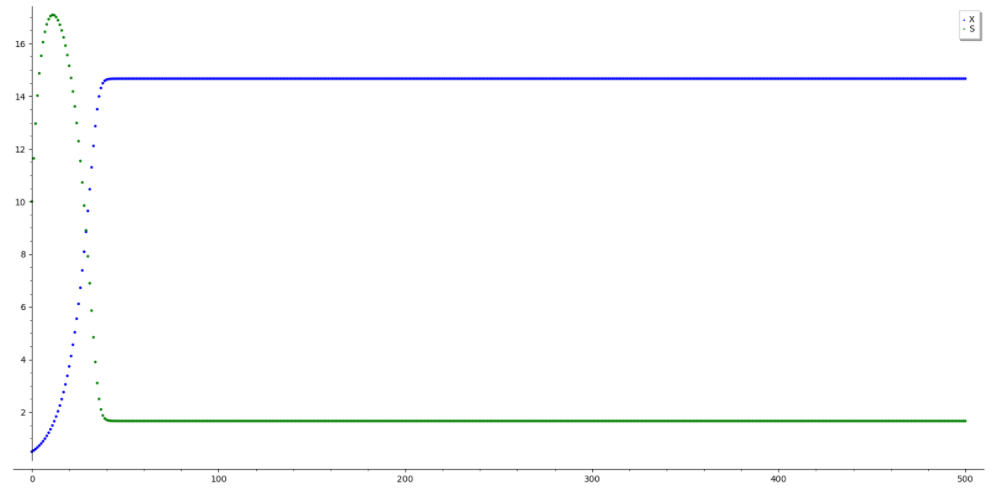
\includegraphics[scale=0.4]{Modelo_9.png}} 
        \caption*{Aumentando a concentração de massa celular em 10 vezes}
\end{figure}
\vspace{-7mm}
\begin{itemize}
\begin{AutoMultiColItemize}
    \item $\mu_{max} = 1.6$ \\
    \item $K_s = 1.0$ \\
    \item $Y = 0.8$ \\
    \item $S_f = 20$ \\
    \item $D = 1.0$ \\
    \item $X_0 = 0.5$ \\
    \item $S_0 = 10.0$ \\
    \item $\mu = 1.0$ 
\end{AutoMultiColItemize}
\end{itemize}
\end{frame}

\begin{frame}{}
\begin{figure}[H]
        \centering
        \hbox{\hspace{0.0em} 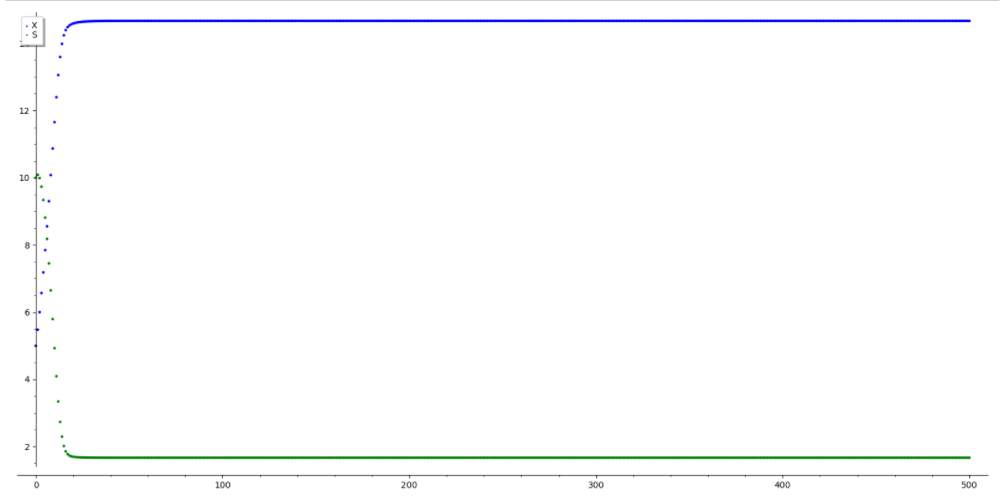
\includegraphics[scale=0.4]{Modelo_10.png}} 
        \caption*{Aumentando a concentração de massa celular em 100 vezes}
\end{figure}
\vspace{-7mm}
\begin{itemize}
\begin{AutoMultiColItemize}
    \item $\mu_{max} = 1.6$ \\
    \item $K_s = 1.0$ \\
    \item $Y = 0.8$ \\
    \item $S_f = 20$ \\
    \item $D = 1.0$ \\
    \item $X_0 = 5.0$ \\
    \item $S_0 = 10.0$ \\
    \item $\mu = 1.0$
\end{AutoMultiColItemize}
\end{itemize}
\end{frame}

\begin{frame}{}
\begin{figure}[H]
        \centering
        \hbox{\hspace{0.0em} 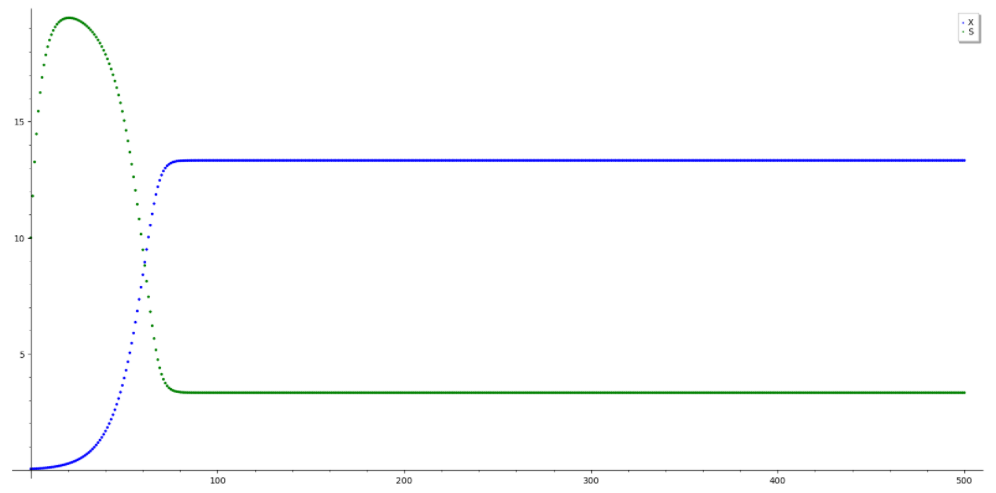
\includegraphics[scale=0.4]{Modelo_11.png}} 
        \caption*{Dobrando a constante de saturação}
\end{figure}
\vspace{-7mm}
\begin{itemize}
\begin{AutoMultiColItemize}
    \item $\mu_{max} = 1.6$ \\
    \item $K_s = 2.0$ \\
    \item $Y = 0.8$ \\
    \item $S_f = 20$ \\
    \item $D = 1.0$ \\
    \item $X_0 = 0.05$ \\
    \item $S_0 = 10.0$ \\
    \item $\mu = 1.0$
\end{AutoMultiColItemize}
\end{itemize}
\end{frame}

\begin{frame}{}
\begin{figure}[H]
        \centering
        \hbox{\hspace{0.0em} 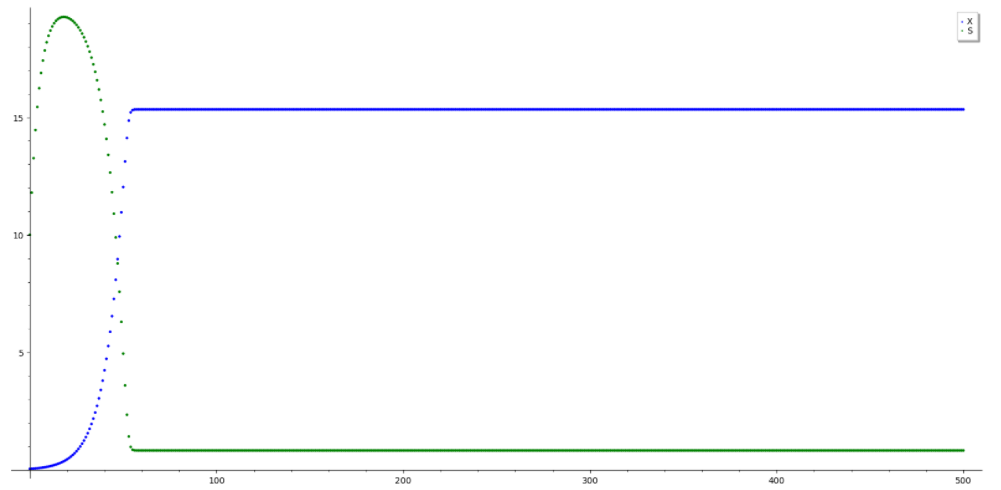
\includegraphics[scale=0.4]{Modelo_12.png}} 
        \caption*{Diminuindo a constante de saturação pela metade}
\end{figure}
\vspace{-7mm}
\begin{itemize}
\begin{AutoMultiColItemize}
    \item $\mu_{max} = 1.6$ \\
    \item $K_s = 0.5$ \\
    \item $Y = 0.8$ \\
    \item $S_f = 20$ \\
    \item $D = 1.0$ \\
    \item $X_0 = 0.05$ \\
    \item $S_0 = 10.0$ \\
    \item $\mu = 1.0$
\end{AutoMultiColItemize}
\end{itemize}
\end{frame}

\begin{frame}{}
\begin{figure}[H]
        \centering
        \hbox{\hspace{0.0em} 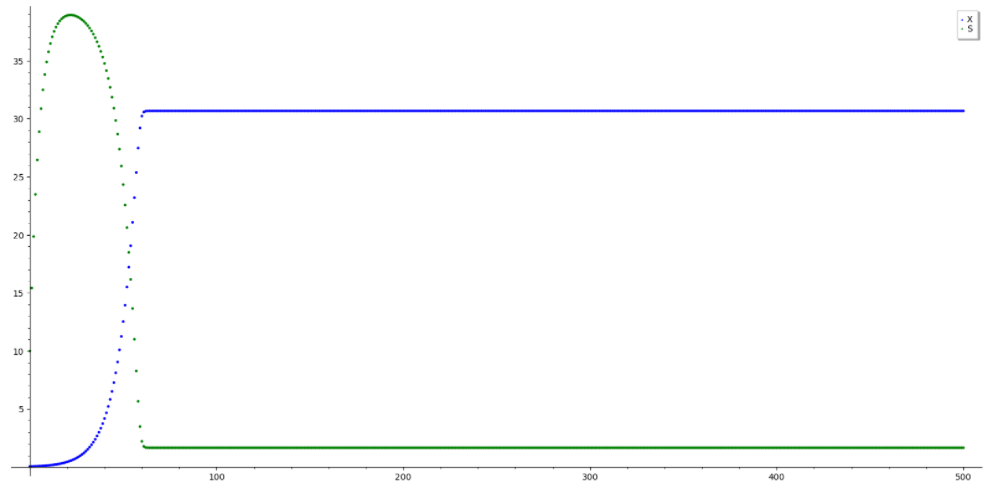
\includegraphics[scale=0.4]{Modelo_13.png}} 
        \caption*{Dobrando o limite de concentração de entrada do substrato}
\end{figure}
\vspace{-7mm}
\begin{itemize}
\begin{AutoMultiColItemize}
    \item $\mu_{max} = 1.6$ \\
    \item $K_s = 1.0$ \\
    \item $Y = 0.8$ \\
    \item $S_f = 40$ \\
    \item $D = 1.0$ \\
    \item $X_0 = 0.05$ \\
    \item $S_0 = 10.0$ \\
    \item $\mu = 1.0$
\end{AutoMultiColItemize}
\end{itemize}
\end{frame}

\begin{frame}{}
\begin{figure}[H]
        \centering
        \hbox{\hspace{0.0em} 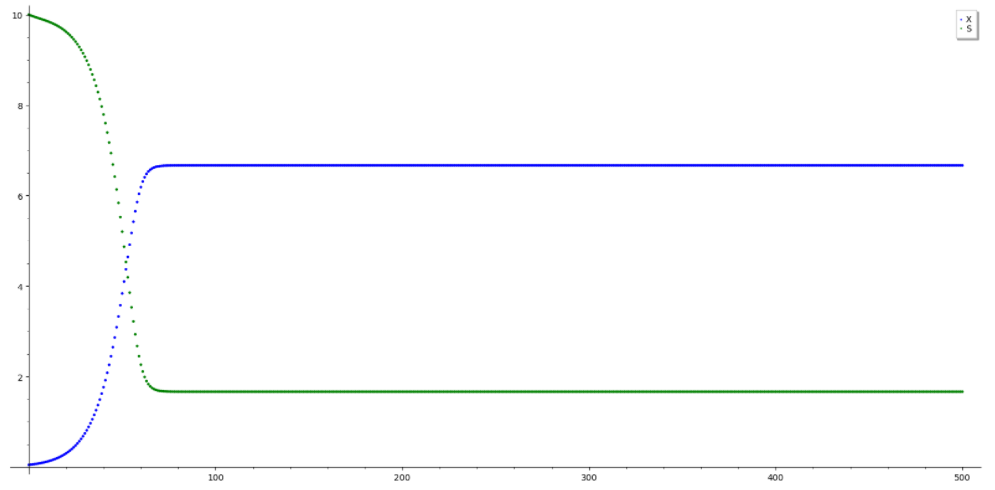
\includegraphics[scale=0.4]{Modelo_14.png}} 
        \caption*{Diminuindo o limite de concentração de entrada do substrato pela metade}
\end{figure}
\vspace{-7mm}
\begin{itemize}
\begin{AutoMultiColItemize}
    \item $\mu_{max} = 1.6$ \\
    \item $K_s = 1.0$ \\
    \item $Y = 0.8$ \\
    \item $S_f = 10$ \\
    \item $D = 1.0$ \\
    \item $X_0 = 0.05$ \\
    \item $S_0 = 10.0$ \\
    \item $\mu = 1.0$
\end{AutoMultiColItemize}
\end{itemize}
\end{frame}

\begin{frame}{}
\begin{figure}[H]
        \centering
        \hbox{\hspace{0.0em} 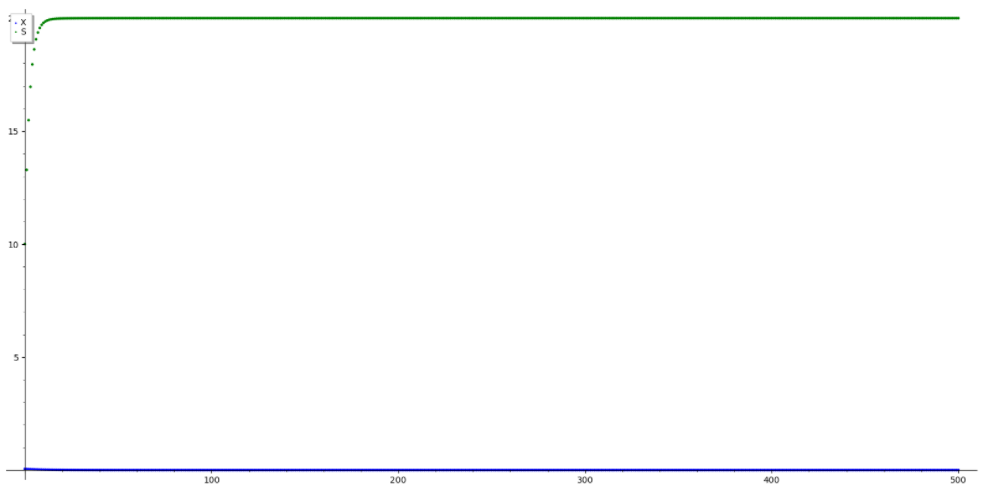
\includegraphics[scale=0.4]{Modelo_15.png}} 
        \caption*{Dobrando a taxa de dilução}
\end{figure}
\vspace{-7mm}
\begin{itemize}
\begin{AutoMultiColItemize}
    \item $\mu_{max} = 1.6$ \\
    \item $K_s = 1.0$ \\
    \item $Y = 0.8$ \\
    \item $S_f = 20$ \\
    \item $D = 2.0$ \\
    \item $X_0 = 0.05$ \\
    \item $S_0 = 10.0$ \\
    \item $\mu = 2.0$
\end{AutoMultiColItemize}
\end{itemize}
\end{frame}

\begin{frame}{}
\begin{figure}[H]
        \centering
        \hbox{\hspace{0.0em} 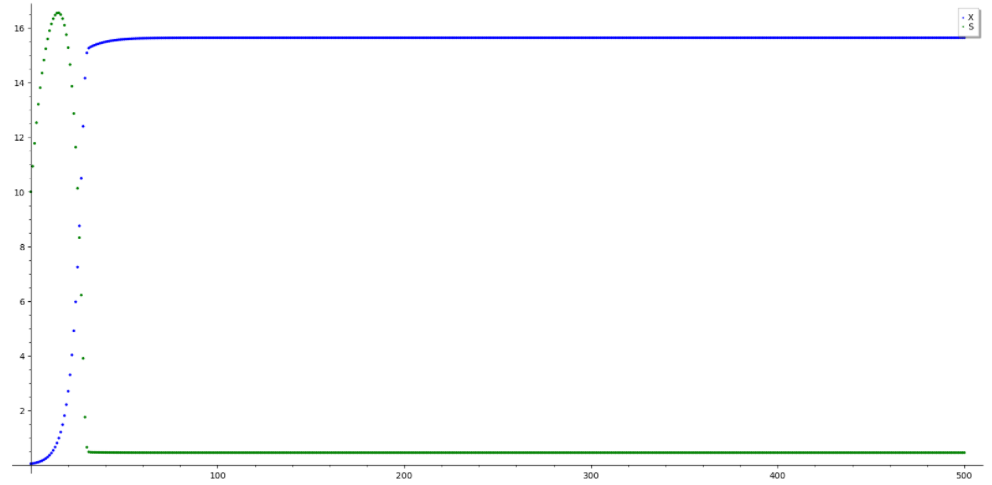
\includegraphics[scale=0.4]{Modelo_16.png}} 
        \caption*{Diminuindo a taxa de diluição pela metade}
\end{figure}
\vspace{-7mm}
\begin{itemize}
\begin{AutoMultiColItemize}
    \item $\mu_{max} = 1.6$ \\
    \item $K_s = 1.0$ \\
    \item $Y = 0.8$ \\
    \item $S_f = 10$ \\
    \item $D = 0.5$ \\
    \item $X_0 = 0.05$ \\
    \item $S_0 = 10.0$ \\
    \item $\mu = 0.5$
\end{AutoMultiColItemize}
\end{itemize}
\end{frame}

\begin{frame}{}
\begin{figure}[H]
        \centering
        \hbox{\hspace{0.0em} 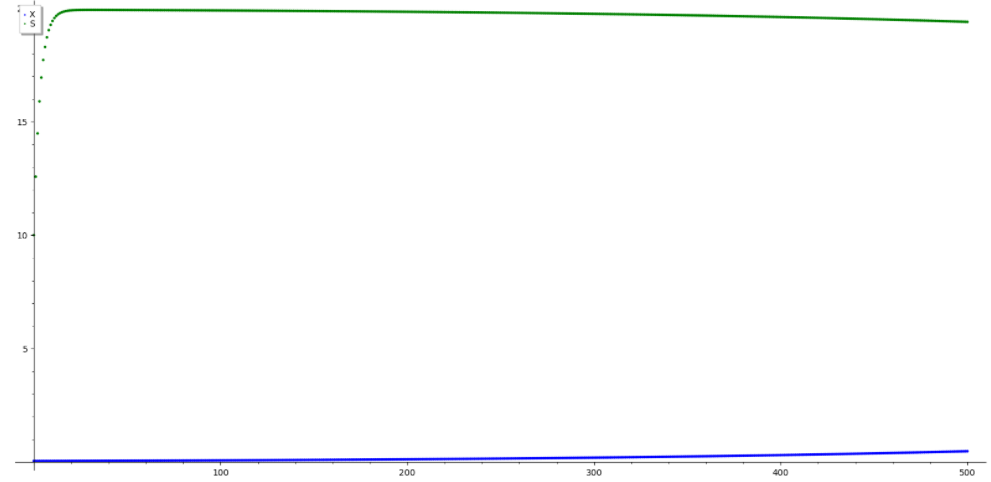
\includegraphics[scale=0.4]{Modelo_17.png}} 
        \caption*{Aumentando a taxa de dilução}
\end{figure}
\vspace{-7mm}
\begin{itemize}
\begin{AutoMultiColItemize}
    \item $\mu_{max} = 1.6$ \\
    \item $K_s = 1.0$ \\
    \item $Y = 0.8$ \\
    \item $S_f = 20$ \\
    \item $D = 1.5$ \\
    \item $X_0 = 0.05$ \\
    \item $S_0 = 10.0$ \\
    \item $\mu = 1.5$
\end{AutoMultiColItemize}
\end{itemize}
\end{frame}

%\begin{frame}{Conclusão}

%\end{frame}

%{\setbeamercolor{palette primary}{fg=black, bg=orange!30} %You can change the colours
%\begin{frame}[standout]
%  Thank you! And thank to yourself because you did all the job. 
%\end{frame}
%}
%\appendix

% Esse tipo de slide não conta pra tabela de conteúdos 
%\begin{frame}{Back up}
%    These slides won't appear in the table of contents and will not be %counted as the total slides.
%\end{frame}

\end{document}
